\chapter{Einleitung}
\addthumb{Einleitung}{\huge{\textbf{\thechapter.}}}{white}{haw_rot} 

Im Jahr 1926 veröffentlitche der Wirtschaftswissenschaftler Nikolai D. Kondratieff (* 1892, \dag 1938) die Theorie \glqq Die Langen Wellen der Konjunktur\grqq \cite{hensen:gesundeGesellschaft}.
Leo Nefiodow erweiterte 2006 die Theorie, damit die Entwicklung des 20. Jahrhunderts einfließen konnte.\\
Kontratieff zeigte, dass sich die gesellschaftliche Wandlung nicht willkürlich vollzog. Seit der Industrialisierung Mitte des 18. Jahrhunderts stand der Wohlstand der Gesellschaft in direkter Beziehung zu besonderen Erfindungen. Er betrachtete die Phasen des Wohlstandes und die direkt folgende Wirtschaftskrise und entdeckte die später nach ihm benannten \glqq Kontratieff-Zyklen\grqq.
Wie in Abbildung \ref{zyklen} zu sehen ist, war die Dampfmaschine die erste Basisinnovation\footnote{Basisinnovationen müssen nach Nefiodow vier Eigenschaften erfüllen: Entstehung eines neuen Marktes mit vielen Arbeitsplätzen; Innovation bestimmt den Zyklus; Basisinnovationen haben einen Zyklus von 40 - 60 Jahren; Sie bestimmen die Entwicklungsrichtung} und revolutionierte die Textilindustrie.\cite{wieden:liquidwork}

%\begin{wrapfigure}{c}{10cm}
%\centering
%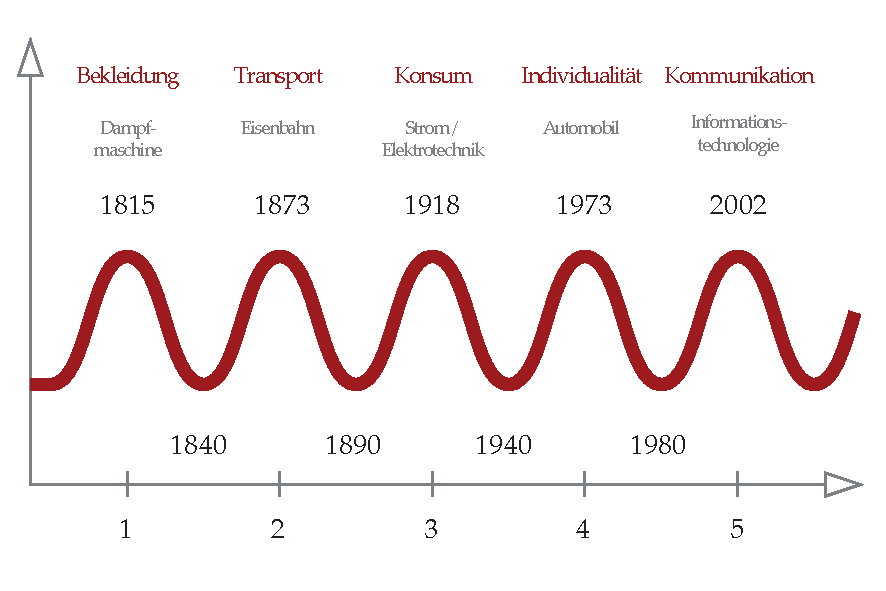
\includegraphics[width=8cm]{./img/zyklen.pdf}
%\caption{Kontratieff Zyklen}
%\label{zyklen}
%\end{wrapfigure}

\begin{figure}[htbp]
  \vspace{0.5cm}
  \centering
  \fbox{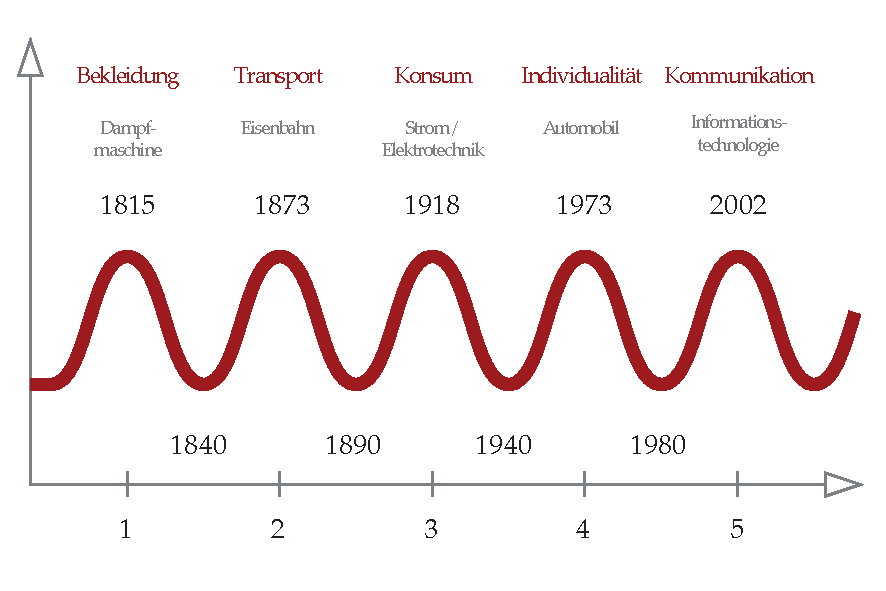
\includegraphics[angle=0,width=12cm]{./img/zyklen.pdf}}
  \caption{Kontratieff-Zyklen}
  \label{zyklen}
  \vspace{0.5cm}
\end{figure}

Diese Erfindung gilt als Beginn des ersten Kontratieff-Zyklus. Vor dem maschinellen Betrieb wurden Spinnräder noch manuell bedient und Kleidung war teuer. Die dampfbetriebenen Webstühle steigerten
die effizient um das 200-fache. In 20er Jahren stagnierte die Branche, da die Rohstoffbeschaffung und Warenverteilung das Maximum der Effizienz erreicht hatte. Mit der Erfindung der Eisenbahn gelang der Übergang vom ersten in den zweiten Zyklus. In den folgenden Jahren konnte nun das Bedürfnis nach verbesserten Transportmöglichkeiten gestillt werden.\\
Dampfmaschine, Eisenbahn, Strom, Motor und der Mikrochip stehen alle für eine Basisinnovation, die zukünftige Gesellschaften geprägt haben. Im lauf der Zeit verschwinden die Erfindungen aus dem Bewusstsein der Menschen und werden zu Gegenständen des Alltags. Motor und Mikrochip sind so stark im gesellschaftlichen Leben verankert, dass Sie nicht mehr direkt wahrgenommen werden. Betrachtet man eine elektrische Zahnbürste, ist es selbstverständlich, dass die Energie aus dem Stromnetz bezogen wird und der Bürstenkopf von einem Motor angetrieben wird.\\
Das Jahr 2002 gilt als Höhepunkt des fünften Kontratieff-Zyklus und die Gesellschaft befindet sich gerade im Übergang zum Sechsten. Noch fehlt die aktuelle Basisinnovation und auch das zu stillende Bedürfnis ist nach der Kommunikation noch nicht bestimmt.\\
Nach Nefiodow \cite{nefiodow:gesundheit} gibt es vier Möglichkeiten welcher Markt in Zukunft den sechsten Kontratieff prägen wird:
\begin{itemize}
  \item \textbf{Informationsmarkt} \\
  		Mobile Geräte und Soziale Netzwerke sind maßgebend für diesen Markt. So verhalf der Kurznachrichtendienst Twitter zum sogenannten \glqq Arabischen Frühling\grqq, durch die blitzschnelle Kommunikation über das Netz\footnote{http://www.heise.de/tr/blog/artikel/Wie-funktioniert-die-Twitter-Revolution-1761481.html \\aufgerufen am 06.01.2014}.
  \item \textbf{Bio - und Nanotechnologie} \\
  		Die Erfindung des Mikroskops und die Entschlüsselung der DNA im Jahr 2000 gilt als Basisinnovation. Anfangs wurden die Erkenntnisse nur in Medizin und Pharmazie angewendet. Heute profitiert auch die Landwirtschaft und Lebensmittelindustrie davon.
  \item \textbf{Umwelttechnologie}
  		Auch der Bereich der Umwelttechnologie sorgte für einen Zuwachs an Arbeitsplätzen. In Deutschland standen im Bereich der erneuerbaren Energien 170.000 Menschen in einem Beschäftigungsverhältnis\footnote{vgl. \cite{nefiodow:gesundheit} S. 107}.
  \item \textbf{Gesundheit}
  		Der Gesundheitsmarkt vereint technologische Komponenten wie die Medizintechnik und psychosoziale Gesundheit. Es erfolgt ein Wechsel vom heutigen \glqq Krankheitswesen\grqq zum Gesundheitswesen, angefangen von der Burnout-Prophylaxe, Gesundheitstourismus zur Bionik und künstlichen computergesteuerten Prothesen.
\end{itemize}

\section*{Gesundheit als sechster Kontratieff-Zyklus}

Nach Granig\cite{nefiodow:gesundheit} ist der Gesundheitsbereich der derzeit am schnellsten wachsende Markt\footnote{Gemessen am Anteil der Branche am Bruttoinlandsprodukt}. Die Bevölkerung ist gewillt in die eigene Gesundheit zu investieren und die Unternehmen positionieren sich im Gesundheitsbereich (Siemens beispielweise verstärkt sich im Bereich der Medizintechnik).
Die Bio- und Nanotechnologie ist und die Medizintechnik ähneln sich in einigen Bereichen. Sowohl Siemon Cord \cite{cord:innovation} als auch Granig\footnote{vgl. \cite{nefiodow:gesundheit} Seite 116 f} sprechen davon, dass der Markt sich nur gehemmt entwickeln kann. Grund dafür sind sowohl in der Nano- und Medizintechnik veraltete Gesetzte und auch ethnische Hürden, die es zu überwinden gilt.\\
Cord schreibt, dass 100\% des Wissens der Biotechnik aus Hochschulwissen stammt (allerdings aufgrund der erwähnten Einschränkungen noch nicht ökonomisch verwertet werden kann). Zwar trifft diese hohe Prozentzahl nicht auf die Medizintechnik zu, da viel Entwicklung in den Unternehmen stattfindet. Doch der Grundstein für Innovation wird bei den Studierenden der Hochschulen und Universitäten gelegt. Die Bildungseinrichtungen werden ein zentrales Standbein für den kommenden sechsten Kontratieff mit dem Schwerpunkt Bio-, Medizintechnik und Gesundheit sein.

\section*{Der Studiengang Biomedizinische Technik}



%Diese Basisinnovationen müssen nach Nefiodow folgende vier Eigenschaften erfüllen.
%\begin{itemize}
%	\item Es entsteht ein neuer Markt mit einer großen Anzahl an Arbeitsplätzen
%	\item Basisinnovationen bestimmen die Entwicklung des Zyklus
%	\item Basisinnovationen haben einen Lebenszyklus von 40 - 60 Jahren
%	\item Sie bestimmen die Entwicklungsrichtung 
%\end{itemize}
